\chapter{DeepTAM\authorB}

This Chapter is based on the work of:"DeepTAM: Deep Tracking and Mapping with Convolutional Neural Networks".\cite{ZUB19a}

\section{What is DeepTAM?}
DeepTAM provides a keyframe-based dense camera tracking and depth map estimation system that is entirely learned. The idea of DeepTAM is based on DTAM \cite{dtam}.The generic idea is: drift-free camera tracking via a dense depth map towards a keyframe and aggregation of depth over time. But the way to implement this concept is different. In the DeepTAM deep networks are used for tracking and mapping.These networks learn only from data. It also processes more than two images for the 6 DOF egomotion and depth estimation. With that it can avoid the drift of the use of keyframes and as more keyframes come in it can refine the depth map.

\section{Tracking}
The main objective is to estimate a 4 x 4 transformation matrix T. This matrix maps a point in the keyframe coordinate system to the coordinate system of the current camera frame. DeepTAM uses an more efficient way. It generates a virtual keyframe and tries to predict the increment instead of trying to estimate T. For more details see \cite{ZUB19a}. 

\subsection{Network Architecture}

\begin{figure}[h]
	\centering
	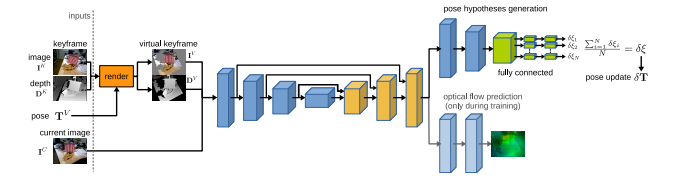
\includegraphics[width=1.1\textwidth]{./media/images/DeepTAM_schematic.PNG}
  	\caption{Schematic of DeepTAM
  	\\Source: \url{http://lmb.informatik.uni-freiburg.de/Publications/2019/ZUB19a}}
  	\label{DeepTAMschematic}
\end{figure}

To estimate the 6 DOF pose between a keyframe and an image the encoder-decoder-based architecture is used. To estimate camera motion you have to relate the keyframe to the current image. Because of that DeepTAM uses optical flow as an supportive task. With this optical flow the network is ensured to take advantage of the relationship between both frames. It uses two network branches for predicting the pose. One is the optical flow prediction and the other is the pose hypotheses generation. This improves the accuracy for the pose prediction.

\section{Mapping}

DeepTAM computes a set of depth maps every keyframe. For good quality depth maps, information will be accumulated in a cost volume. From this cost volume the depth map will be extracted by means of a convolutional neural network.
\newline
\newline
Normally the cost volume is taken as data term and because of that a depth map can be obtained by searching for the minimum cost. Using this method, because of the noise in the cost volume, there must be various optimization techniques and sophisticated regularization terms included to extract the depth in a robust manner.DeepTAM instead has a network which is trained to use the matching cost information in the cost volume and simultaneously combine it with the image-based scene priors to obtain more accurate and more robust depth estimates. 
\newline
\newline
The accuracy is limited by the number of depth labels for cost-volume-based methods. That is why there is an adaptive narrow band strategy used to keep number of labels constant while increase the sampling density. The cost volume for the narrow band recomputes for a small selection of frames and searches again for a better depth estimate. The narrow band requires a good initialization and regularization to keep the band in the right place but allows to recover more details in the depth map.

\begin{figure}[h]
	\centering
	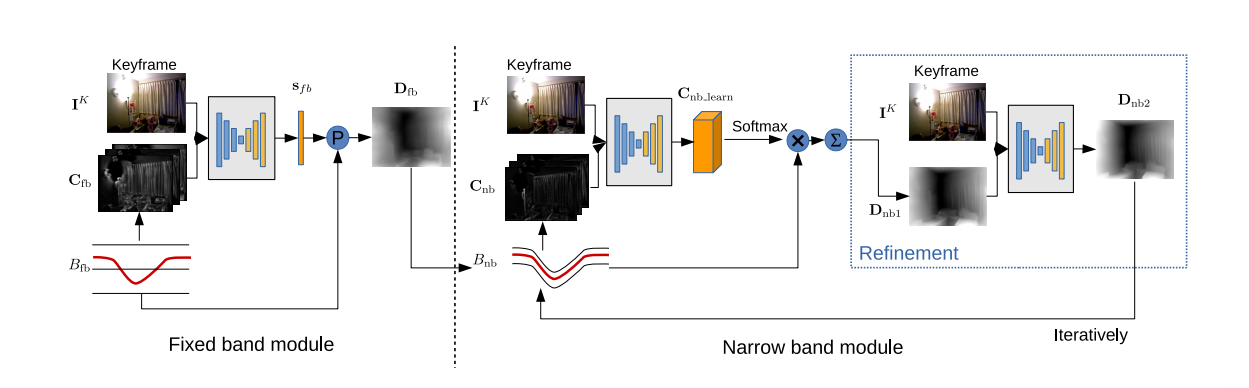
\includegraphics[width=1.1\textwidth]{./media/images/DeepTAM-Mapping.PNG}
  	\caption{Mapping Networks Overview
  	\\Source: \url{http://lmb.informatik.uni-freiburg.de/Publications/2019/ZUB19a}}
  	\label{DeepTAM-Mapping}
\end{figure}

\subsection{Network Architecture}
The network is trained to predict the keyframe inverse depth from the keyframe image and the cost volume which is computed from a set of images and camera poses. The keyframe inverse depth is represented as inverse depth, which enables a more precise representation with closer distance. There is also a coarse-to-fine strategy along the depth axis applied. Mapping is divided into a fixed band module and a narrow band module. The narrow band cost volume centers at the current depth estimation and accumulates information in a small band close to the estimate, while the fixed band module builds a cost volume with depth labels evenly spaced in the whole depth range.
\newline
\newline
Between the minimum and maximum depth label the fixed band module regresses an interpolation factor as output. Because of this the network cannot reason about the absolute scale of the scenes, which makes the network more flexible and generalize better. The fixed band contains a set of fronto-parallel planes as depth labels. Conversely the narrow band contains discrete labels which are individual for each pixel.The prediction of interpolation factors is not useful since the network in the narrow band module has no knowledge of the band’s shape. The narrow band is not provided with the band shape, because the network tends to ignore the cost information in the cost. This makes the depth regularization difficult. Therefore there is another network appended, which focuses on this problem.

\subsection{Training}
In about 8 days in total the training of the mapping network can be acomplished on a NVIDIA GTX 1080Ti.

%\gls{optical-flow}



